%%%%%%%%%%%%%%%%%%%%%%%%%%%%%%%%%%%%%%%%%%%%%%%%%%%%%%%%%%%%%%%%%%%%%%%%%%
%%%%%%%%%%%%   CAPTER 3   %%%%%%%%%%%%%%%%%%%%%%%%%%%%%%%%%%%%%%%%%%%%%%%%
%%%%%%%%%%%%%%%%%%%%%%%%%%%%%%%%%%%%%%%%%%%%%%%%%%%%%%%%%%%%%%%%%%%%%%%%%%
\chapter{Software Design}
\label{chap:software_design}

As mentioned in the previous chapter, we will focus on the challenges faced when utilizing the domain name system. Before we discuss data transport through the hierarchical name system in the section\ref{sec:software_design:tx}, we will look at the data collection and ID generation (\ref{sec:software_design:data_collection}).\\
Section \ref{sec:software_design:ref_impl} demonstrates how we realized the proposed solutions in the reference implementation.

%%%%%%%%%%%%%%%%%%%%%%%%%%%%%%%%%%%%%
%%%%%%%%%%%%%%%%%%%%%%%%%%%%%%%%%%%%%
%%%%%%%%%%%%   SECTION   %%%%%%%%%%%%
%%%%%%%%%%%%%%%%%%%%%%%%%%%%%%%%%%%%%
%%%%%%%%%%%%%%%%%%%%%%%%%%%%%%%%%%%%%
%\section{Parameter}
%\label{sec:measurement:parameter}

%

%\newpage


%%%%%%%%%%%%%%%%%%%%%%%%%%%%%%%%%%%%%
%%%%%%%%%%%%%%%%%%%%%%%%%%%%%%%%%%%%%
%%%%%%%%%%%%   SECTION   %%%%%%%%%%%%
%%%%%%%%%%%%%%%%%%%%%%%%%%%%%%%%%%%%%
%%%%%%%%%%%%%%%%%%%%%%%%%%%%%%%%%%%%%
\section{Data Collection}
\label{sec:software_design:data_collection}
    As we have shown in \ref{subsec:related:pii} and \ref{subsec:related:law} it is wise to avoid the collection of PII. While it may be avoidable for the statistical data and numeric values, this might not be possible for the generated ID.\\
    The ID should be unique to identify a device persistent over reboots and system updates but do not allow to conclude a device.
    While the gathered data needs to be useful to the purpose of the collection, the collection practices need to be compliant according to privacy laws. 
    
 %
    %%%%%%%%%%%%%%%%%%%%%%%%%%%%%%%%%%%%%
    %%%%%%%%%%%% Subsection %%%%%%%%%%%%%
    %%%%%%%%%%%%%%%%%%%%%%%%%%%%%%%%%%%%%
    %
    \subsection{Data selection}
        \label{subsec:software_design:selection}
        To get the most out of data collection, it needs to be relevant to the task it has to fulfill.
        While a wide range of collected metrics might help  broaden the view over the monitored landscape, it may hinder the evaluation and detection of relevant data points. Therefore data collection should always be kept to a minimum needed to help the cause for the collection.\\
        Users are more willing to share nonsensitive information, as Woldaregay et al.   \cite{woldaregay_user_2020} have shown for medical data, Ziefle et al.  \cite{ziefle_users_2016} for data sharing on social networks, and Leon et al.  \cite{leon_what_2013} for sharing information with online advertiser. Furthermore, Schneegrass et al.  \cite{10.1145/3290605.3300753} have shown that the willingness of information sharing for sensory data is based on a positive or negative connotation of the data in question.\\
        
        As we discuss Internet-connected data collections, there is always the possibility for a data breach, or an adversary actor, who may target the collected data. If PII is contained in the data set, the possible yield for an attacker is higher compared to public, non personally identifiable data.\\
        To protect the devices and thereby the users' identity, numerical data should always be collected in bins or ranges.\\
        The exact amount of available memory in a system provided in byte or even kilobyte may fingerprint a device. IP and MAC addresses are sensitive data and should not be collected at all, as these could be connected to other Internet-related activities and lead to an attack on the user, to gain control over their device. \\
        As the National Academies of Science, Engineering and Medicine propose in their Consensus report \cite{groves_federal_2017}, the more attributes are included in a data set, the likelier the re-identification of individuals and the greater the threat for external data linking.\\
        
        Before collecting data large scale, a project should define the intent behind the process. With a clear outline of objectives, relevant parameters can be identified. 
        Therefore we propose a minimal data collection set containing only relevant information to fulfill the purpose of the collection as recommended by NIST and OECD.\\
        To be open about the collected information, the current state of the collection should be easily available to any user, as well as the reasoning for the collection of each date.
        Following NIST's recommendations again, these data sets should be reviewed on a regular basis to validate that each date is still needed.\\
        
        The objective for an open source project could be to reduce the number of defects in the released software or to collect usage statistics to improve the development of the software for a given target. A combination of objectives is possible as well.\\
        Based on the objectives, a list of parameters can be compiled to retrieve data relevant to the purpose.
        To, e.g., detect system crashes, the time since the last reboot (uptime) of a given device may be relevant, as well as the amount of memory available and the CPU or System on Chip. Further on, the software version in use needs to be included in this example. These are all non-PII and may be collected without further obfuscation. As we have stated before, it is recommended to classify numeric values, like available memory, into categories.\\
        
        Although the collected information does not need to be obfuscated, the user should be made aware of the data collection. In some cases, user acknowledgment might be required as well. Therefore banner, push notifications, or notifications on installation or first execution should be shown to the user. \\
        In the case of a Linux distribution, this could be done by a pop-up message on the first login to a graphical screen or using a banner on a remote or serial login to the device.
        The GDPR requires that consent must be given specific and may be withdrawn at any time \cite{noauthor_gdpr_2020}.\\ 
        Therefore a Linux distribution might require to click or set a value to enable and disable the data collection. An IoT firmware, like Tasmota, might need to enable data collection via a web interface for a device. This needs to be done before any user information is collected\\. 
        
        Furthermore, an organization should provide a privacy policy for the data collection, even if no PII is collected. It should state which information is collected and transmitted on a given device.\\
        This could be seen as good faith and increase the users' trust in the data collection program. If private information is collected, a privacy policy is required by GDPR. Another important point to keep in mind is that user might want to remove their data from the collection later. If the collected data contains PII, it might fall under the GDPR's right to be forgotten jurisdiction. The user should be able to ask for deletion, if he no longer consents with the collection.
        This makes an identifier an important factor to recognize the user's data. It needs to be available to exert the user's right to remove the data from a collection.
        
          
    \subsection{ID generation}
        \label{subsec:software_design:id}
        To keep the actions required by the user to participate to the minimum feasible, ID generation should be an automated process without the need for the user to register for data collection. There are some registration processes available like Kluczniak et al. show in  \cite{kluczniak_anonymous_2015} that provide a robust way to separate the user data from the token used to sign-up. This would require the user to actively register for the collection process, which would most likely reduce the number of users participating.\\
        
        The ID generation is based on hardware information available to identify devices on a reliable and reproducible basis. Therefore, it is persistent through a reboot, a re-flash, or an update.\\
        We recommend the use of the available MAC addresses. These should be hashed individually and combined into one string which is then hashed again. Both hashing operations should be done with a strong cryptographic hashing function.
        As there are several different hash functions out there, the hashing should be one-way and un-keyed. A one-way hash function (OWHF) fulfills the requirements for a hash \textbf{\textit{h}} function, which can be seen in equation \ref{eq:hash} \cite{sobti_cryptographic_2012}.
        
        \begin{equation}
            \label{eq:hash}
            \textbf{h} : D \longrightarrow R
        \end{equation}
        
        where domain $D = \{0,1\}^*$ and $R=\{0,1\}^n$ for $n >= 1$.

\newpage

        In addition, an OWHF must meet five requirements defined by Merkle in  \cite{merkle_secrecy_1979}.
        \begin{itemize}
            \item \textbf{\textit{h}} must be applicable to any length of data blocks
            \item A fixed length output is created by \textbf{\textit{h}}
            \item A message digest \textbf{\textit{h}}(x) with \textbf{\textit{h}} and x given is easy to compute
            \item If \textbf{\textit{h}} and \textbf{\textit{h}}(x) are known, it is computationally infeasible to find x
            \item If \textbf{\textit{h}} and \textbf{\textit{h}}(x) are known, it is computationally infeasible to find x and x' so that $\textbf{\textit{h}}(x) = \textbf{\textit{h}}(x')$
        \end{itemize}
        
        This function should come from the Secure Hash Algorithm 2 or 3 (SHA-2/SHA-3) family. While SHA512 is the stronger function and is recommended, it is not available on all devices.\\
        A single MAC consists of 48 bits, from which 24 bits are vendor-specific and equal in all devices from this vendor. The other 24 bits are a unique identifier for a given network interface. As most internet-connected devices come with pre-installed/soldered network interfaces, this could lead to brute force attempts to regenerate the MAC address from a hash. Especially on hardware with only one physical network interface. With the power jump in recent graphic card generations, a hash based only on 24 unique bits can be brute-forced in a concise time \cite{tirado_new_2018}. Therefore the generated hash needs to be enhanced.\\
        
        There are some well-known ways to enhance security on stored passwords and similar tasks. Three of them are PBKDF2 \cite{kaliski_pkcs_2000}, Bcrypt \cite{provos_future-adaptable_1999} and Scrypt \cite{josefsson_scrypt_2016}.
        Bcrypt is a key derivation function (KDF) based on the Blowfish block cipher. It receives a number of inputs, like iteration count, input password, and salt. The password is limited to 56 bytes, and the iteration count \textit{n} results in $2^n$ bcrypt iterations. It is designed to be secure through being memory and storage complex \cite{hatzivasilis_password_2015-1} \cite{provos_future-adaptable_1999}.\\
        Scrypt is also a password-based key derivation function designed to be computational complex to increase the costs of hardware-based attacks. It creates a key from a list of inputs that define the cost of the function.\\
        These key derivation functions have two use cases. On the one hand, they are used for password hashes in modern operating systems, protecting the user's password against easy access \cite{percival_stronger_nodate}. 
        The other use case is the derivation of a key based on a token and another key \cite{camenisch_privacy_2011}. Attacking a KDF in itself is not feasible. An attacker would need to iterate over a range of passwords or regular expressions and apply the KDF to them \cite{percival_stronger_nodate}.\\
        Another example of such a derivation function is Password-Based Key Derivation Function 2 (PBKDF2). A pseudo-random function is applied to a given password and salt for a number of iterations. 
        Salting reduces its vulnerability against brute force and dictionary attacks. An adversary either starts guessing passwords and applies the function to its guesses or uses a set of rules or words from a list. Rainbow table attacks, which utilize precompiled hash tables, are made less feasible with salting as well, and the computation time is increased significantly \cite{kaliski_bkaliskirsasecuritycom_pkcs_2000}. \\
        While Scrypt is designed to be an expensive function to break for an attacker, it is also the most resource-demanding function during the creation of the key, reducing its usability for embedded devices. Bcrypt is also computational intense and therefore resistant against attack from ASICs or GPUs. PBKDF2 is only a small circuit implementation and requires the lowest amount of RAM, which makes it best suited for embedded devices while reducing its effectiveness against brute force attacks on ASICs or GPUs \cite{hatzivasilis_password_2015-1}.\\

        To keep IDs reproducible, we need to derive our input password and salt from data provided by the device, which won't alter during a reinstall of a system. For devices with nonvolatile flash memory, the Memory Technology Devices (MTD) are usually devices with solid-state file systems \cite{giometti_mtd_2017} \cite{woodhouse_memory_nodate}. These partitions can contain configuration information for wireless devices. This contains device-unique data, which is ideal to use as key and/or salt.\\
        
        To further strengthen the ID against brute-forcing and decreasing the amount of character used in a DNS query, the generated ID should be reduced to a feasible number of bytes. Hereby the number of expected users should be in relation to the selected byte length of the ID.\\
        The available numbers of variation may be calculated for given string length \textit{n} and length of alphabet \textit{k} as seen in equation \ref{eq:variations}.
        \begin{equation}
            \label{eq:variations}
            V(n;r) = n^{r}
        \end{equation}

        As DNS limits the available alphabet to [a-z][0-9] this would fix \textit{n} to $26 + 10 = 36$.
        
        To calculate the probability of a hash collision, we can utilize equation \ref{eq:base_prob_hash}
        
        \begin{equation}
             \label{eq:base_prob_hash}
             P(k,V) = 1 - \exp{\frac{-k(k-1)}{2 \cdot V}}
        \end{equation}
     
        Based on  \cite{preshing_hash_2011} equation \ref{eq:base_prob_hash} can be simplified for expected collisions probabilities of $\frac{1}{10}$ or less and large k to
     
        \begin{equation}
            \label{eq:simp_prob_hash}
            P(k,V) = \frac{k^2}{2V} 
        \end{equation}

\newpage

        The generated IDs should have a low collision probability rate to keep them unique but should be selected small enough to keep the bytes used in a DNS request low. \\
        To calculate a possible number of hashes with a given probability \textit{P}, we can transform equation \ref{eq:simp_prob_hash} to a reduced quadratic equation.
        \begin{equation*}
            0 = k^2 - 2PN
        \end{equation*}
        which can then be solved as seen in equation \ref{eq:solvek}
        \begin{equation}
            \label{eq:solvek}
            k = \sqrt{2PN}
        \end{equation}
        
        With equation \ref{eq:solvek} it is possible to calculate the amount of supported user/devices before the risk for a hash collision reaches the threshold.
\newpage



%%%%%%%%%%%%%%%%%%%%%%%%%%%%%%%%%%%%%
%%%%%%%%%%%%%%%%%%%%%%%%%%%%%%%%%%%%%
%%%%%%%%%%%%   SECTION   %%%%%%%%%%%%
%%%%%%%%%%%%%%%%%%%%%%%%%%%%%%%%%%%%%
%%%%%%%%%%%%%%%%%%%%%%%%%%%%%%%%%%%%%
\section{Data Transmission}
\label{sec:software_design:tx}
%
    While the ID is generated to be transmitted over DNS, the collected data is still in plain text and a large chunk of text. As we have shown in \ref{subsec:related:dns} only 63 byte long labels, up to a total of 255 bytes for a complete request are supported.
    Therefore the data needs to be encrypted to provided privacy during the transport and chunked and transformed to allow transport over DNS.\\
    %
    %%%%%%%%%%%%%%%%%%%%%%%%%%%%%%%%%%%%%
    %%%%%%%%%%%% Subsection %%%%%%%%%%%%%
    %%%%%%%%%%%%%%%%%%%%%%%%%%%%%%%%%%%%%
    %
    \subsection{Data Encryption}
        \label{subsec:software_design:encryption}
        The collected data should never be transported unencrypted over the internet to provide privacy and security to the client. An attacker might be able to monitor the DNS request send by the client and use the contained information to figure out possible weaknesses of the system in use from them and maybe available additional information. \\
        In comparison to the generated ID, where we rely on the irreversibility of the result, the encryption of the data needs to be reversible to perform statistical analysis on them.
        Again the load on the user should be minimal. Therefore we would recommend an automated system again.\\
        A well-known system for secure data transport is TLS, which is used in modern HTTPS implementations. TLS utilizes asymmetric encryption, also known as public-key encryption. 
        Thereby a publicly available key, the public key, is used to encrypt the data on one side by anyone. On the other hand, the private key is usually only available at one instance, which decrypts messages encrypted with the public key. In TLS, asymmetric cryptography is used in key exchange algorithms to agree on session keys, which then, in turn, are used for symmetric encryption once the session build-up is complete \cite{noauthor_how_nodate}.\\
        As there should be no session build-up between the client and the collecting server to keep the sender's anonymity intact, we recommend asymmetric encryption.
        One of the most employed asymmetric encryption systems is the Rivest-Shamir-Adleman algorithm (RSA). They proposed procedures with the following four properties \cite{rivest_method_1978}.
        \begin{itemize}
            \item The encryption procedure \textit{E} and the decryption procedure \textit{D} are both easy to compute.
            \item Only \textit{D} can decrypt messages encrypted with \textit{E}. When \textit{E} is published, there is no easy way to compute \textit{D} from it
            \item Deciphering an enciphered Message \textit{M} results in \textit{M}. \textit{D(E(M)) = M}
            \item \textit{E(D(M)) = M}, which means that a message \textit{M} that is first deciphered and then enciphered results in \textit{M}
        \end{itemize}
        This procedure from 1978 is still valid today. Therefore we recommend creating a  public/private key pair for asymmetric encryption.\\
        An RSA key can have a length of up to 4096 bit. While Debian, Fedora, and CACert have moved to 4096-bit sized keys \cite{pocock_rsa_nodate}, NIST recommends keys with at least 2048 bit size \cite{barker_transitioning_2019}. Keys of at least 2048 bit length stand unbroken at the time of writing and are therefore recommended for the client data as well. 
        Next to RSA, there are three other algorithms used for key generation. 
        These are the Digital Signature Algorithm (DSA), Edwards-curve Digital Signature Algorithm (EdDSA), and Elliptic Curve Digital Signature Algorithm (ECDSA) \cite{mody_comparing_2020}.
        Support for DSA has been dropped from OpenSSL 7.0 onwards by default, as it has some known weaknesses if the randomness used to generate the key (nonce) is not random enough. The same issue is faced by ECDSA effectively taken these two algorithms out of consideration \cite{miller_ecdsa_2020}.
        EdDSA uses elliptic curves to provide security like ECDSA instead of key lengths like RSA and DSA. But unlike ECDSA, it does not rely on a random number. It generates its nonce deterministically as a hash. The elliptic curve 25519 has been adopted as the standard
        in the public-key signature algorithm Ed25519. It is one of the few elliptic curves to provide sufficient security \cite{mody_comparing_2020}.\\
        This leaves either RSA $\geq$ 2048 bit or Ed25519 as a public-key signature algorithm.
        While RSA is widely supported, EdDSA has a better performance and provides the same level of security with smaller keys \cite{mody_comparing_2020}.\\
        
        The generated public key can be shared over the TXT record of a domain. Each of these records is expected to hold at least 255 bytes, so a key might be split up over multiple TXT records if its length exceeds this size.
        The client software should then be able to query the TXT records of a given domain and retrieve the public key that way.
        The retrieved key can be utilized to encipher the collected data in a fashion that the server can decrypt it with the private key. Another advantage of this system is that the key pair can be exchanged at any point in time if the private key got compromised.
        
     %
    %%%%%%%%%%%%%%%%%%%%%%%%%%%%%%%%%%%%%
    %%%%%%%%%%%% Subsection %%%%%%%%%%%%%
    %%%%%%%%%%%%%%%%%%%%%%%%%%%%%%%%%%%%%
    %
    \subsection{Fitting data to DNS request}
        \label{subsec:software_design:fitting}
        Since elements from the domain name system are required to support [a-z], [0-9], and hyphens only, the data needs to be transformed to a format that can be transmitted reliably. Upper case letters are hereby treated the same as lower case ones.
        For example, EXAMPLE.COM. would lead to the same result as example.com. and ExAmPlE.com.
        Therefore a base 32 encoding would be feasible to keep the transmission size as low as possible. In addition, it offers the widest set of supported symbols while using only one symbol that DNS does not support. The equal sign is used as a padding character, which needs to be exchanged with a hyphen to make it conforming. The hyphen can be used as a padding symbol, as it is not present in the RFC 4648 base 32 alphabet \cite{josefsson_simonjosefssonorg_base16_2006}. Base 16 encoding would reduce the number of available symbols below the supported range of symbols. In contrast, base 64 encoding would add additional symbols, which are not supported in the domain name system. These are the plus '+' and slash '/' symbol. Base 64 keeps the equal sign for padding, which makes a DNS conform substitution harder.\\
        A URL and filename safe base 64 alphabet variant is mentioned in RFC 4648 as well, which replaces the plus sign with the minus and the slash symbol with an underscore while keeping '=' as the padding character. Again this makes a valid substitution hard and unnecessary as all relevant symbols are already covered in the Base 32 alphabet \cite{josefsson_simonjosefssonorg_base16_2006}.\\
        
        As the number of the available bytes is limited to 63 per DNS label and limited to a total of 255 bytes, the collected and encrypted data needs to be split up into multiple chunks and multiple messages.\\
        The base (\textbf{B}) of every message should be composed as \textbf{B} $=$ $<$optionally sub-domain$>$.$<$domain$>$.$<$TLD$>$.
        Followed by an identifying section \textbf{I} $=$ $<$device id$>$-$<$current message number$>$-$<$total messages in a block$>$. 
        The remainder of available bytes is used for the encrypted data message split up in up to 63-byte large chunks \textbf{M}.
        The final message is composed as \textbf{M}.\textbf{I}.\textbf{B}. The shorter \textbf{B}, the more bytes are left for \textbf{I} and \textbf{M}. \textbf{I} should be selected reasonable long to address the number of expected user.\\
        
        It needs to be ensured that every part of the query conforms with the Base 32 encoding or lower to be compliant with every DNS server implementation \cite{mockapetris_domain_1987}.

\newpage


%%%%%%%%%%%%%%%%%%%%%%%%%%%%%%%%%%%%%
%%%%%%%%%%%%%%%%%%%%%%%%%%%%%%%%%%%%%
%%%%%%%%%%%%   SECTION   %%%%%%%%%%%%
%%%%%%%%%%%%%%%%%%%%%%%%%%%%%%%%%%%%%
%%%%%%%%%%%%%%%%%%%%%%%%%%%%%%%%%%%%%
\section{Reference Implementation}
\label{sec:software_design:ref_impl}
    To showcase how this data collection can be utilized, we developed dalec \cite{venz_ikstreamdalec_2021}.
    In the following, we will discuss our selection and how we implemented the transport of the collected data.
%
\subsection{Data Collection}
    The purpose of collecting data on the OpenWrt platform is the improvement of the distribution and a general survey of the systems in use. For this purpose, we decided to collect the data in the following list. 
    \begin{itemize}
        \item Software version
        \item Available and total RAM (in $2^n$ categories)
        \item System uptime
        \item CPU data:
        \begin{itemize}
            \item Model
            \item Model name
            \item System type
            \item Machine Info
            \item Vendor ID
            \item Core and Thread count
        \end{itemize}
        \item Kernel version
        \item Architecture
    \end{itemize}
    
    The software version is added for automated evaluation, and allows defining which data points are collected, as this may change over different versions. RAM size allows for the classification of devices. This enables the project to see if the usual system utilizes only a small amount of memory or runs at its capacity.\\
    The uptime date shows if a system needs regular reboots or can run for a longer period of time. The CPU data can be used to get a hint on system types and if certain systems are more represented than others. The architecture allows to further specify the collected CPU information.\\
    With the kernel information collected, it is possible to see if the users adopt new OpenWrt updates or keep their system on a version for an extended time.\\
    
    We decided to implement dalec to keep its storage footprint low and extract the information from files if available. This was possible for all data points, except for the architecture, which could only be gathered through the \textit{uname} command. The data is stored in a log file placed under \textit{/tmp/dalec} so that a user can review the information collected about the system. The collection process is started every four hours and transmitted to a configured server. It is only enabled if the user runs the command prompted during installation. A random backoff time was added to every start. While we only aim for one measurement point per day, there is no way for the server to tell the client if a transmission was successful or complete. Therefore we transmit the data several times a day. The random backoff helps to prevent hitting a coincidental network congestion every time, hindering the data transmission.\\
    The collection tool is extensible to allow additional data collection to assist debugging in the OpenWrt forum. The client, however, will only transmit the data listed above. The tool is written in POSIX conforming shell script to allow the usage on a wide range of devices and be usable as well, where packaging is not possible.
%
\subsection{ID generation}
    To generate a unique ID for a given device, we collect all available MAC addresses of physical devices and hand them to the \textit{OpenSSL sha3-512} digest function. These hashes are concatenated into one string, which is then hashed again. We call this our ID. As we go for \textit{OpenSSL} as a dependency for PBKDF2, we use its \textit{SHA512} digest function to generate stronger hashes than the available \textit{sha256} function available in OpenWrt by default. The resulting hash is then passed to the encrypt function of \textit{OpenSSL} utilizing \textit{aes256-cbc} and PBKDF2 with 10.000 iterations and SHA512 as derivation digest.\\
    PBKDF2 was selected, as it can be run, even with a high iteration count, in reasonable time on low-end hardware \cite{ertaul_implementation_2016}. For encryption aes256 was selected as it is fast, even on older devices and has low RAM requirements. Furthermore it provides good security and stands unbroken at the time of writing. There are some known attacks against AES  \cite{schneier_another_2009} \cite{lu_new_2008} \cite{bernstein_cache-timing_nodate} \cite{biryukov_key_2009}, but none of them are computationally feasible with foreseeable hardware. In 2003 the NSA validated the use of AES with either 192 or 256 key lengths for encryption of all information up to TOP SECRET confidentiality \cite{noauthor_national_2003}.\\
    
    The salt and key for the password based key derivation depend on the device's hardware. If MTD partitions are available, we hash the \textit{art, factory, u-boot}, and/or \textit{u-boot-env} partitions and use the first 16 bytes of the resulting hash as salt. The remaining bytes are used as the key. If no such partitions are available, the ID, generated in the previous step, is used for salt and key. The first 16 bytes are used as a salt, while the remainder of the ID forms the key. While this is not optimal, keeping save IDs consistent over multiple flashes, overwrites, and reboots it's a necessary step. An attacker would still need to recreate the base hash and then apply the encryption function to it. This process is time and resource intense.\\
    
     We further enhanced the brute-forcing protection in reducing the generated hash to the last 32 bytes and removed all special symbols from the resulting string, which leaves around $36^{32} = 6.33x10^{49}$ possible variations. While this makes it nearly impossible to recreate the original ID and MAC address, the probability of a hash collision increases due to the reduced number of available hashes. A simplified process description can be seen in figure \ref{fig:id_gen}\\
     
     \begin{figure}
         \centering
         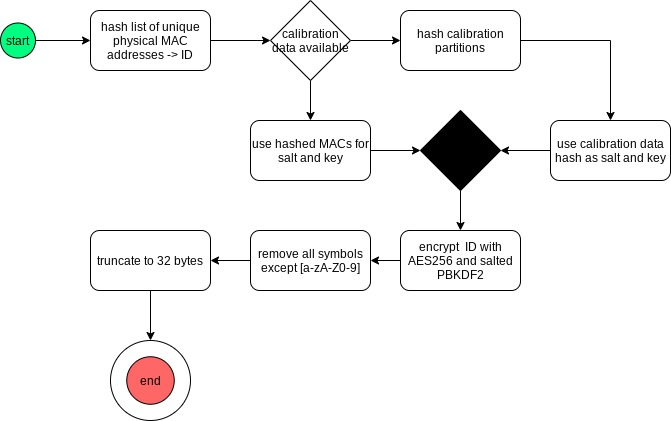
\includegraphics[width=\textwidth]{latex/figures/id_generation.jpg}
         \caption{Overview of the simplified ID generation process}
         \label{fig:id_gen}
     \end{figure}
    
     As we have shown in section \ref{subsec:software_design:id} we can calculate the number of available hashes with a given collision probability. For this system, we want to keep the collision probability below $P = 10^{-18}$ for $N = 36^{32}$ possible hashes.
     Based on equation \ref{eq:solvek}, we can calculate the number of hashes \textit{k}, that can be assigned.
     
     \begin{equation*}
         k = \sqrt{2PN}
     \end{equation*}
     
     \begin{equation}
        \label{eq:k1018}
         k = \sqrt{2 \cdot  10^{-18} \cdot 36^{32}}
     \end{equation}
     
\newpage     

     Equation \ref{eq:k1018} resolves to around $1.13x10^{16}$ possible IDs before we reach the probability of $10^{-18}$ for a collision. If we assumed that every available IPv4 address ($2^{32} = 4,294,967,296)$ would use dalec, this would be more than enough.\\
     
     We allow uppercase letters to be included in a generated ID. This information might or might not be preserved through the message traversal through the domain name system. We change any uppercase letter to lower case on the server-side. 
     As we have collected the data and generated an ID, we need to process and transmit the information next.
     
     
% 
\subsection{Information processing}

    As \textit{base32} is packaged in C\textit{coreutils} in OpenWrt, we decided to go for a base16 encoding instead. This is available with \textit{hexdump}, which is included in the default \textit{busybox} OpenWrt configuration. While this increases the number of messages needed to be sent, it reduces the footprint for dalec. The collected data is read from a temporary file, in which the data is stored as key-value pair. Only the value for each key is taken and separated by a semicolon to reduce the amount of data transmitted. This increases the overhead on the server-side, but as we transmit the client version in our transmission, each field can be sorted to a key.\\
    The generated, colon-separated values, string is then passed to \textit{OpenSSL} for encryption. To encrypt the message, we need to collect the server's public key first.
    This is acquired by querying the TXT record of a domain. We decided to go for an RSA 4096 bit key as it is widely adopted, where Ed25519 might not be supported by all target systems.\\
    Therefore we split the key into three records. Each is prefixed with a position identifier, as multiple queries might not return the TXT records in the same order.\\
    After encryption, the data is base 64 encoded for easier storage on the server-side and put into hexdump for base 16 encoding.\\
    The encoded string is then separated into 62 byte-sized chunks. These chunks are combined with our base domain and the ID message number combination, allowing up to three chunks to be transmitted at one time. A simplified overview of the process can be seen in figure \ref{fig:data_proccess}\\
    
    \newpage
    
    \begin{figure}[h!]
        \centering
        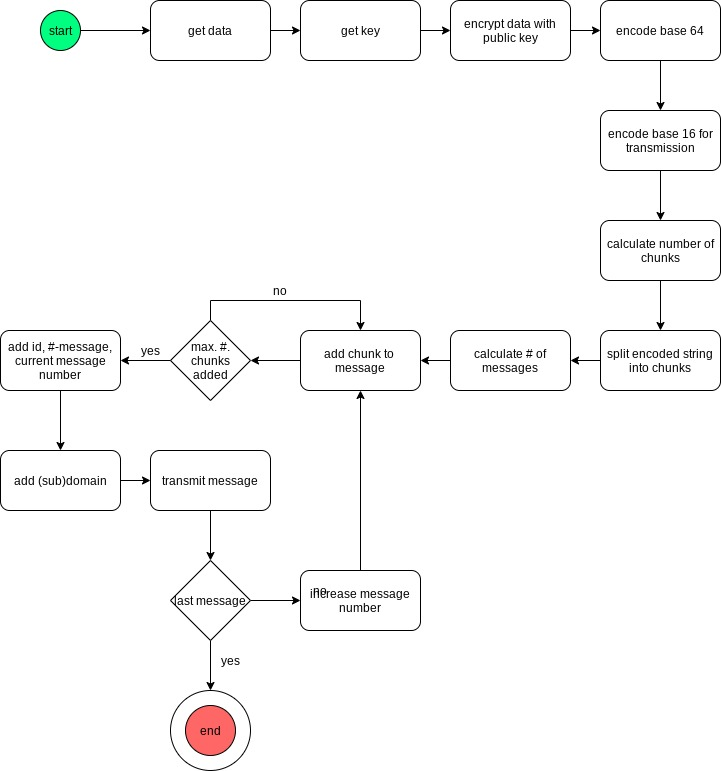
\includegraphics[width=\textwidth]{latex/figures/data_processing.jpg}
        \caption{Data processing overview}
        \label{fig:data_proccess}
    \end{figure}
    
    \newpage
    
    To send out the DNS queries, we use \textit{drill}, which has a reduced storage footprint (\SIlist{19}{\kilo\byte}) compared to \textit{bind-dig} (\SIlist{41}{\kilo\byte}). If dependencies are included in the calculation, the difference is even bigger. While drill adds \textit{libldns} (\SIlist{100}{\kilo\byte}), \textit{bind-dig}
    adds \textit{bind-libs} (\SIlist{879}{\kilo\byte}), which makes bind-dig consume \SIlist{801}{\kilo\byte} more storage space than drill as can be seen in table \ref{tbl:size_comp}. For the ease of comparison, mutual dependencies are not considered.\\
    
    \begin{table}[h]
        \centering
        \caption{Size comparison of drill and bind-dig with dependencies}
        \label{tbl:size_comp}
        \begin{tabular}{llll}
            Packagename & Size & Packagename & Size  \\
            \hline
            drill       & \SIlist{19}{\kilo\byte}   & bind-dig    & \SIlist{41}{\kilo\byte} \\ 
            libldns     & \SIlist{100}{\kilo\byte}  & bind-libs   & \SIlist{879}{\kilo\byte} \\
            \hline\hline
                        & \SIlist{119}{\kilo\byte}  &             & \SIlist{920}{\kilo\byte} \\
                        &      &             &      
        \end{tabular}
    \end{table}
    
    Removing all debug information from the dalec scripts during the build process of the OpenWrt package, we were able to reduce their size to \SIlist{10.1}{\kilo\byte} overall in version 0.1.5.
    

    
%%%%%%%%%%%%%%%%%%%%%%%%%%%%%%%%%%%%%
%%%%%%%%%%%%%%%%%%%%%%%%%%%%%%%%%%%%%
%%%%%%%%%%%%   SECTION   %%%%%%%%%%%%
%%%%%%%%%%%%%%%%%%%%%%%%%%%%%%%%%%%%%
%%%%%%%%%%%%%%%%%%%%%%%%%%%%%%%%%%%%%
\section{Summary}

This chapter discussed the client-side data collection application and the data transmission concept. We presented how to utilize the DNS system to transmit the user data and demonstrated the need for encryption before transferring through the network.
We also introduced the reference implementation for our proposed solution. It was shown how dalec uses encryption not only for the user data, but also in the ID generation process. Furthermore, dalec's preprocessing pipeline was illustrated. We also discussed the dependency selection with the intention in mind to keep dalec's storage footprint minimal.
In the next chapter, we will discuss the server-side of data collection.
%